\documentclass{article}
\usepackage{amsfonts,amsmath,amsthm,amssymb,mathtools,xcolor,array,enumerate,setspace,graphicx,tikz,multicol}
\usepackage[margin=1in]{geometry}
\setlength\parindent{0pt} 
\title{Homework 9}
\author{MA372 Introduction to Discrete Math}
\date{Due: Lesson 29 08 APR 2022}

\begin{document}
\maketitle 

\textbf{Instructions.} Solve the following problems on material up through Lesson 27. Your solutions should be typeset using \LaTeX\, for final submission and include a coversheet.\\

Note: Graphs may be included in your submission as images using the graphicx package along with the command \textbackslash includegraphics\{ \}. If you wish to create your graphs using \LaTeX, see the links under ``Creating Graphs Using TikZ'' in the LaTeX Resources folder on Blackboard.

\begin{enumerate}
	\item For each of the following relations, determine if it is reflexive, symmetric, antisymmetric, and/or transitive. Explain your answers.
	\begin{enumerate}[a)]
		\item On the integers $\mathbb{Z}$, define the relation $R=\{(a,b)|\text{ }a-b\text{ is odd}\}$.
		\item On the set of all bit strings of length four, define the relation $T$ where $rTs$ if and only if the sum of the characters in $r$ equals the sum of the characters in $s$.
	\end{enumerate}
	
	\item On the set $\{0,1,2,3\}$, define the relation $R=\{(0,0),(0,1),(1,1),(1,1),(1,2),(2,2),(2,3)\}$. For this relation,
	\begin{enumerate}[i.]
		\item represent the relation as a zero-one matrix,
		\item represent the relation as a directed graph, and
		\item determine whether the relation is reflexive, symmetric, antisymmetric, and/or transitive.
	\end{enumerate}
	
	\item Determine the relation on the set $A=\{1,2,3,4,5\}$ given by the zero-one matrix
	\[\begin{bmatrix}
			1 & 0 & 1 & 0 & 1\\0 & 1 & 1 & 0 & 0\\0 & 1 & 1 & 0 & 0\\1 & 0 & 0 & 1 & 1\\0 & 0 & 0 & 1 & 1
		\end{bmatrix}.\]

	\item Determine the relation on the set $\{1,2,3,4,5\}$ given by the digraph below.
	\begin{center}
		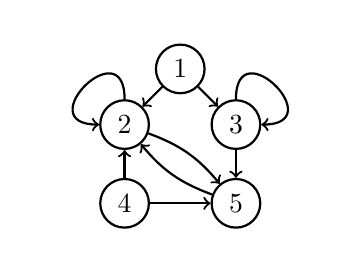
\begin{tikzpicture}[node distance={10mm}, thick, main/.style = {draw, circle}] 
			\node[main] (1) {1}; 
			\node[main] (2) [below left of=1] {2}; 
			\node[main] (3) [below right of=1] {3}; 
			\node[main] (4) [below of=2] {4}; 
			\node[main] (5) [below of=3] {5}; 
			\draw[->] (1) -- (2); 
			\draw[->] (1) -- (3); 
			\draw[->] (3) -- (5);
			\draw[->] (4) -- (2);
			\draw[->] (4) -- (5);
			\draw[->] (2) to [out=90,in=180,looseness=5] (2); 
			\draw[->] (3) to [out=90,in=0,looseness=5] (3);
			\path[->]
				(2) edge[bend left=15] (5)
				(5) edge[bend left=15] (2);
		\end{tikzpicture}
	\end{center}
	
	\item Show that the relation $\mathbb{Z}$ defined by $R=\{(a,b)|\text{ 2 divides }a-b\}$ is an equivalence relation and describe the distinct equivalence classes of the relation.
	
	\item Let $A=\{0,1,2,3,4\}$.
	\begin{enumerate}[a)]
		\item Do the sets $\{0,1\},\{2,4\},\{1,3\}$ form a partition of $A$? Explain your answer.
		\item Determine the equivalence relation on $A$ induced by the partition $\{0\},\{1,3,4\},\{2\}$.
	\end{enumerate}

\end{enumerate}

\end{document}
